\documentclass[12pt, a4paper, openany, oneside]{book}
\usepackage[italian]{babel}
\usepackage[T1]{fontenc}
\usepackage[utf8]{inputenc}
\usepackage{amsmath} 
\usepackage{xcolor}
\usepackage{listings}
\usepackage{hyperref}
\usepackage[margin=1in]{geometry}
\usepackage{graphicx}
\graphicspath{{./img/}}
\definecolor{britishracinggreen}{rgb}{0.0, 0.26, 0.15}
\newcommand\tab[1][1cm]{\hspace*{#1}}
%usepackage[latin1]{inputenc}
\begin{document}
%\pagestyle{plain}
\author{\href{https://github.com/daverhapsody}{DaveRhapsody} \and Jacopo De Angelis \and DlcGold}
\title{Linguaggi di Programmazione}
\color{blue}
\date{30 Settembre 2019}
\color{black}
\maketitle
\tableofcontents
\chapter{Introduzione al corso}
\section{Programma del corso}
Il corso è volto ad insegnare dei paradigmi di programmazione dei seguenti tipi:
\subsection{Logica Matematica e Linguaggi logici (Prolog)}
Termini, fatti(predicati), regole, unificazione, procedura di risoluzione
\subsection{Linguaggi funzionali e Lisp (et al.)}
Atomi, liste, funzioni e ricorsione
\subsection{Linguaggi imperativi} % (fold)
\label{sub:linguaggi_imperativi}
Memoria, stato, assegnamenti, puntatori
\\ 
{\color{black} \rule{\linewidth}{0.3mm} }
\\
Il concetto è che con questo corso si vanno a studiare paradigmi più evoluti,
usati tutt'ora e comunque aventi un ampio approccio logico, oltretutto LISP è 
usato nelle pagine web (Si userà moltissimo la ricorsione, A I U T O)
\section{Modalità d'esame}
\label{sec:modalità_d_esame}
\subsection{subsection name}
\label{sub:subsection_name}
\begin{itemize}
	\item il voto finale sarà una media pesata dei voti conseguiti nell'esame 
	relativo alla parte teorica e nell'esame del progetto 
	\begin{itemize}
		\item Occhio, il peso è a discrezione dei prof
	\end{itemize}
\end{itemize}
\subsection{Prove parziali}
\label{sub:prove_parziali}
Le prove d'esame sono costituite da uno scritto di 6-10 domande, e da un 
progetto da consegnare entro una data prefissata
\section{Appelli regolari}
\label{sec:appelli_regolari}
Gli appelli regolari sono composti da un progetto ed un esame scritto, che può
essere seguito da un esame orale a discrezione del docente basato sui temi 
trattati durante il corso
\\
\textbf{NON C'E' POSSIBILITA' DI RECUPERI}, infatti scritto, orale e progetto 
vanno sostenuti \color{red} \textbf{NELLO STESSO APPELLO} \color{black}
\\
Progetto e scritto sono corretti separatamente
\paragraph{NON CI SARANNO ECCEZIONI}
\label{par:non_ci_saranno_eccezioni}
Lo avete già letto nel passaggio precedente, ma lo ripeto lo stesso perchè 
deve essere chiaro che N O N  S I  F A N N O  E C C E Z I O N I.
%------------------------------------------------------------------------------
\chapter{Il paradigma}
\section{Cos'è?}
E' il metodo di soluzione ad un determinato problema, a seconda dei paradigmi si
hanno diversi tipi di linguaggi di programmazione
\subsection{Storicamente}
Il primo paradigma è l'imperativo, cioè il paradigma basato sui tre costrutti
di selezione, iterazione e sequenza. \\
Inoltre si mantiene il concetto di assegnamento di un valore ad una determinata variabile
\subsection{L'effetto collaterale}
Viene definito effetto collaterale quando, a seguito dell'esecuzione di un qualsiasi
codice, il contenuto di un'area di memoria viene cambiato; per intenderci, anche
solo l'istruzione "x += 1" genera un effetto collaterale, poichè nell'area di 
memoria di x viene cambiato il valore. \\
Perchè è importante tutto ciò, direte. Semplice: il paradigma puro funzionale si 
basa proprio sul fatto che un programma non generi mai, mai, \emph{M A I}, effetti 
collaterali.
Successivamente vedremo che in Prolog ci saranno parecchi problemi se provassimo
ad assegnare direttamente un valore ad una variabile
\section{Logica del primo ordine}
Prolog è costituito da una serie di clausole derivanti dalla logica del primo
ordine
\section{Linguaggi funzionali}
Questi si basano proprio sui concetti matematici di funzione, ad esempio si 
ragiona sui domini, sui codomini, sull'insiemistica, solite cose. La loro caratteristica
è che ogni funzione, dato sempre lo stesso input, restituisce sempre lo stesso
risultato. Cosa vuol dire questo? Che non dipende da variabili esterne (e da qui
l'importanza degli effetti collaterali, evitati nei linguaggi funzionali).
%------------------------------------------------------------------------------
\section{Paradigma imperativo}
Le caratteristiche essenziali dei linguaggi imperativi sono legate all'architettura 
di Von Neumann, costituita dai famosi due componenti 
\textbf{Memoria (componente passiva) e Processore (componente attiva)}
\\
In pratica la principale attività che ha la cpu è quella di eseguire calcoli
ed assegnare valori alle variabili, che sono delle celle di memoria.
\paragraph{Va considerato}
Il concetto di variabile è un'astrazione di una cella di memoria, per dire 
se giochi su assembly vai a toccare i veri e propri registri, mentre su C o 
Assembly si ragiona per nome di variabile, non vai di indirizzamento fisico
%------------------------------------------------------------------------------
\subsection{Il concetto di variabile}
In Prolog e LISP cambia completamente il concetto di variabile, ma per come 
saranno presentati vedremo che non c'entra niente. \\
In matematica abbiamo il concetto di variabile? Sì, quella che sta dentro una
funzione, in informatica è diciamo diverso, non è un'astrazione, ma lo vedremo
in seguito
\section{Modello di Von Neumann}
Per manipolare la memoria utilizzo la variabile, simbolo che indica la cella 
di memoria, nei linguaggi funzionali sarà possibile usare il concetto di 
variabile matematica. 
\\ \\
Alla fine il modello di Neumann è composto da I/O, Memoria e CPU con i suoi 
cicli di clock
\section{Stile prescrittivo}
Un programma scritto in un linguaggio imperativo prescrive le operazioni che
la CPU deve eseguire per modificare lo stato di un sistema \\ \\
Le istruzioni sono eseguite nell'ordine in cui queste appaiono, ad eccezione
delle strutture di controllo
\paragraph{Realizzati} sia attraverso interpretazione che compilazione, nati
più per manipolazione numerica che simbolica.
\\
\section{Concetto di programma}
Un programma è intendibile come un insieme di algoritmi e di strutture dati
ma la struttura di un programma consiste in
\begin{itemize}
	\item Una parte dichiarativa in cui son presenti le dichiarazioni di tutte
	le variabili del programma e del loro tipo
	\item Una parte che descrive l'algoritmo risolutivo utilizzato, mediante istruzioni del linguaggio	
\end{itemize}
\section{Perchè utilizzare paradigmi diversi?}
Per esempio l'intelligenza artificiale si sviluppa su linguaggi di 
programmazione specifici, bisogna usare linguaggi che operino in un 
determinato modo, considerati tipo di Altissimo super mega galatticissifantastico 
livello infatti, utilizzabili pure da non programatori
\\ \\
Infatti son generati per manipolazione simbolica non numerica 
\section{Paradigma logico}
Concetto primitivo: Deduzione logica, avente una base di logica formale e un 
obbiettivo, che è intendibile come formalizzazione del ragionamento
\\ \\
\textbf{Programmare infatti significa} descrivere il problema con frasi 
(Formule logiche) del linguaggio, \\
Interrogare il sistema, che effettua deduzioni in base alla "conoscenza 
rappresentata" 
\paragraph{Ai lettori} Mi rendo conto che non si capisca un cazzo, voi 
immaginatevi come mi stia sentendo al momento io mentre prendo appunti.. 
Perdonatemi
\\ \\
Prolog è un insieme di formule ben formate, ragiona con il linguaggio logico, 
con una descrizione della realtà di interesse, di fatto è una dimostrazione in 
un linguaggio logico che costituisce un programma. Più semplicemente ho una  
frase da dare al mio interprete, Prolog icchè fa? Semplicemente la realizza  
sotto forma di dimostrazione. 
\\ 
\section{Esempio di un programma Prolog}
Ci sono fondamentalmente:
\begin{itemize}
	\item Asserzioni incondizionate (\color{red} fatti \color{black})
	A.
	\item Asserzioni condizionate (\color{red} regole \color{black})
	A :- B, C, D, ... , Z.
	\begin{itemize}
		\item A è la conclusione o conseguente (deve avere una sola clausola)
		\item B, C, D, \dots,Z sono le premesse o antecedenti 
	\end{itemize} 
	\item Un'\color{red}interrogazione \color{black} ha la forma: :- K, L, M, 
	\dots, P. \\
\end{itemize}
Ovviamente A, B, C, *TUTTE LE ALTRE*, sono semplicemente predicati
\\
MI RACCOMANDO MASSIMA ATTENZIONE ALLA SINTASSI, ogni clausola Prolog termina
con un punto. \\ \\
La ',' si legge come AND
\subsection{Esempio:}
Due individui sono colleghi se lavorano per la stessa ditta/azienda
\color{red} Regole \color{blue} Fatti \color{black} Interrogazione
\\ \\
\color{red}
collega(X, Y) :-  \\	
\tab lavora(X, Z), \\	
\tab lavora(Y, Z), \\	
\tab diverso(X, Y).
\\ \\
\color{blue}
lavora(ciro, ibm)  \\
lavora(ugo, ibm)  \\
lavora(olivia, samsung)  \\
lavora(ernesto, olivetti)  \\
lavora(enrica, samsung)
\\ \\
\color{black}
:- collega(X, Y). 
\\
{\color{black} \rule{\linewidth}{0.3mm} }
\\
Programmare Prolog non è come scrivere in un linguaggio di programmazione, non
si scrive un algoritmo, in questo caso abbiamo le famose clausole, (regole e 
fatti), 
\paragraph{ATTENZIONE} l'interrogazione non è una clausola, occhio a non confondersi
\subsection{Esempio dell'ordine di una lista}
\begin{itemize}
	\item \textbf{Ordine prescrittivo}: Controlla se la lista è vuota, e dà come 
	risultato la lista vuota stessa, altrimenti calcola una permutazione della 
	lista e controlla se è ordinata, dando come risultato $L_{1}$ altrimenti 
	fa una permutazione su L etc.
	\\
	Il programmatore deve specificare le istruzioni che generano la sequenza 
	di permutazioni della lista L
	$
	\begin{cases}
	$il risultato dell'ordinamento di una lista vuota è la lista vuota $\\
	$Il risultato dell'ordinamento di una lista L e $L_{1} 
	\end{cases}
	$
	Quindi, lo stile prescrittivo presuppone che OGNI SINGOLO CASO venga considerato
	e programmato. non esiste il "ma è ovvio che debba fare questo", ogni singolo
	caso è tua responsabilità. Sì, tua, proprio tu che stai leggendo. Prolog si
	basa su questo tipo di ordine.
	\item \textbf{Stile Dichiarativo}: L'ambiente si fa carico di generare 
	possibili permutazioni della lista L, secondo deduzione matematica
\end{itemize}
\section{Paradigma funzionale}
\begin{itemize}
	\item 
	Si basa sul concetto di funzione matematica, ossia una associazione tra due 
	insiemi che relaziona ad ogni elemento di un insieme (dominio) un solo 
	elemento di un altro insieme (codominio)
	\item La definizione di una funzione specifica dominio, codominio, e regola
	di associazione 
	\\
	\item ESEMPIO: \\
	Incr: N $\to$ N \\
	Incr(x) - x + 1
	\item Dopo aver dato definizione, una funzione è aopplicabile ad un elemento del 
	dominio (argomento) per restituire l'elemento del codominio ad esso associato
	(valutazione)
	\item incr(3) $\to$ 4 
	L'unica operazione utilizzata nel funzionale è l'applicazione di funzioni  
	\item Il ruolo dell'esecutore di un linguaggio funzionale si esaurisce nel 
	calutare l'applicazione di una funzione (il programma) e produrre un valore 
	\item Nel paradigma funzionale puro il valore di una funzione è determinato 
	dagli argomenti che riceve al momento della sua applicazione e non dallo 
	stato del sistema rappresentato dall'insieme complessivo dei valori 
	associati a variabili(e/o locazioni di memoria) in quel momento 
	\item Oggettivamente si ha l'assenza di effetti collaterali \\ \\
\end{itemize}
\paragraph{Attenzione} % (fold)
\label{par:attenzione}
Il concetto di variabile che utilizziamo è quello di "costante" matematica, in 
cui i valori NON sono mutabili, non ho nessun asegnamento
\\ \\
L'essenza della programmazione funzionale consiste nel combinare funzioni 
mediante composizione e uso della ricorsione
% paragraph attenzione (end)
\subsection{Composizione di funzioni + ricorsione} 
La struttura di un programma consiste nella definizione di un insieme di 
funzioni ricorsive mutualmente
\\ \\
L'esecuzione del programma consiste nella VALUTAZIONE dell'APPLICAZIONE di una
funzione principale a una serie di argomenti
\section{LISP}
LISt Processing, \\ \\
Il progretto originale era di creare un linguaggio funzionale puro, infatti
nel corso degli anni sono stati sviluppati molti ambienti di sviluppo lisp
di cui terremo in considerazione Common Lisp e Scheme, oltre che emacs etc.
\subsection{Esempio di programma LISP}
Controlla un elemento se appartiene ad una lista \\ \\
\begin{lstlisting}[language=LISP]
(defun member (item list)) 
(cond ((null list)nil) 
((equal item(first list))T) 
(T(member item(rest list)))) 
(member 42(list 12 34 42))
\end{lstlisting}
Dopo una parentesi tonda ci va per forza una funzione, è fondamentale, defun 
definisce una funzione infatti, dopo c'è il nome di tale funzione. In LISP la 
tabulazione è ESSENZIALE, AUGURI A DISTINGUERE DOVE PORTI LA QUINTA PARENTESI DELLE 
DODICI CHE HAI SCRITTO PIANGENDO SUL CODICE ALLE 2 DI NOTTE.
\\
Gli elementi si separano con lo spazio NON con la virgola, mi raccomando.
\\
La terza riga è la più ostica e dice: è uguale T al primo elemento della lista?
E' molto incastrato ma si riesce a capire, associamo per esempio ad item = 2
(E' un esempio) e list = [1,2] \\
Noi ci arriviamo con la logica che c'è, ma in realtà cosa faremo? Ragioniamo 
per gradi
\begin{enumerate}
	\item null list? \color{magenta} false \color{black}
	\item è 2 = al primo elemento della lista? \color{magenta} False \color{black}
	\item è 2 = al secondo elemento della lista? \color{blue}True \color{black}
\end{enumerate}
Se LISP trova T è come se scrivessimo  \color{blue}\textbf{true}\color{black}
\section{Ambienti RunTime di linguaggi logici funzionali e non}
\begin{itemize}
	\item Richiami di nozioni di architettura e programmazione
	\item Per eseguire un programma di qualsiasi linguaggio il sistema operativo
	deve mettere a disposizione l'ambiente runtime che dia almeno due funzioni
	\begin{itemize}
		\item Mantenimento dello stato della computazione(pc, limiti di memoria)
		\item Gestione memoria disponibile (fisica e virtuale)
	\end{itemize}
	\item L'ambiente runtime può essere una vera e propria macchina virtuale tipo la JVM di java
	\item In particolare la gestione di memoria avviene usando due aree 
	concettualmente ben distinte con funzioni diverse
	\begin{itemize}
		\item Lo stack, ambiente dell'ambiente runtime che serve per la gestione 
		delle chiamate, a procedure metodi etc
		\item L'heap dell'ambiente runtime serve per gestire strutture dinamiche
		\begin{itemize}
			\item Alberi
			\item Liste etc
		\end{itemize}
	\end{itemize}
\end{itemize}
\subsection{Activation frame}
\begin{itemize}
	\item La valutazione di procedure avviene mediante la costruzione sullo
	stack di sistema di activation frames
	\item i parametri formali di una procedura vengono associati ai valori
	(si passa tutto per valore, non esistono effetti collaterali)
	\item E' un altro modo di chiamare i record di attivazione, via
	\item Il corpo della procedura viene valutato (ricorsivamente) tenendo 
	questi legami in maniera statica
\end{itemize}
cioè il concetto è che bisogna capire cosa accade con variabili che risultino 
libere in una sottoespressione
\section{Activation Frame di una funzione}
Contiene:
\begin{itemize}
	\item Return address
	\item Registri
	\item Static / Dynamic link (lo statico punta alle variabili globali)
	\item Argomenti
	\item Local definitions (RV)
\end{itemize}
Se si ha in mente come funziona oggettivamente lo stack (con i record di
attivazione) è la stessa cosa \\
All'esame si potrebbe chiedere cos'è l'activation frame e a icchè serve
\section{Heap e Garbage Collector}
L'heap è l'area di memoria destinata alla memorizzazione delle strutture per i
dati dinamiche, mentre invece il garbage collector ha il compito di accumulare
lo schifo che si accumula tra variabili non deallocate etc, e le dealloca 
appunto.
\chapter{Logica e ragionamento}
Partiamo con le cose semplici, bisogna passare da quello che è un linguaggio 
parlato a una stesura di condizioni \\
Prendiamo un triangolo, vogliamo dimostrare che se due triangoli hanno i due
lati uguali allora è isoscele \\
$$AB = BC \vdash \angle A \angle C$$ 
\begin{enumerate}
	\item AB = BC per ipotesi
	\item ABH = HBC per (3)
	\item Il triangolo HBC è uguale al triangolo HBC ABH per (2)
	\item A e C per (1)
\end{enumerate}
\subsection{Regole di inferenza}
Esempio di una regola di inferenza:
\[
\frac{F_{1}, F_{2}, F_{3}, ..., F_{n}}{R}
\]
\begin{enumerate}
	\item Introduzione della congiunzione (L'AND)
	\item Modus Ponens
	\item Eliminazione della congiunzione
\end{enumerate}
Come lavora il \textbf{Modus Ponens}: \\
E' semplice manipolazione sintattica, osservando la formula che ci vien data
possiamo riscriverla scrivendo come base di conoscenza il conseguente, 
cioè in pratica prendo e sostituisco con il conseguente.
\\ \\
Per far si che le mie formule siano vere, se avessi un A or B può esser vera in 
ben tre casi diversi, non posso eliminare i due casi disgiunti, se voglio 
mantenere una solidità non posso, e quindi questa regola (disgiunzione) non 
esiste.
% consiglio di inserire un'immagine che mostri lo schema del modus ponens
\paragraph{Attenzione} in una dimostrazione non si può dare nulla per 
scontato, tutto cilò che noi diamo per assodato, un pc non lo dà, dobbiamo 
essere molto precisi nelle indicazioni, bisogna lavorare in un'ottica più 
precisa
\\ \\
cerchiamo ora di tradurra tutto in un linguaggio più formale
SE AB = BC E BH = BH e ABH = HBC allora il triangolo ABH è uguale a HBC 
ed abbiamo trasformato (1) in \\ \\
SE triangolo ABH è uguale al triangolo HBC ALLORA AB = BC e BH = BH e AH = HC,
E ABH = HBC E AHB = CHB E A = C
\\ \\
Da un punto di vista formale noi partiamo da un'ipotesi, noi vogliamo 
dimostrare che A = C.
\\ \\
La dimostrazione è un processo sintattico, non ragiono in termini di verità, 
perchè NON si sta parlando di interpretazione ma manipolazione delle formula
\\ \\
Ogni passo deve corrispondere ad una formula, e subito dopo le etichette
\paragraph{Differenza tra assiomi e ipotesi}
Gli assiomi sono conoscenza pregressa del dominio, mentre le ipotesi sono solo
supposizioni iniziali, uno si specifica, l'altro no
\section{Dimostrazione}
E' una sequenza di passi dove il finale è la formula da dimostrare e abbiamo
un insieme di passi intermedi che possono essere presi dalle conoscenze
pregresse, oppure applicando regole di inferenza ai passi PRECEDENTI, solo
precedenti mi raccomando.
\\ \\
Le regole di inferenza sono applicabili solo ai passi precedenti rispetto ad 
una formula
\section{Logica Proposizionale}
Nella logica proposizionale ci si occupa delle conclusioni che possiamo 
trarre da un insieme di proposizioni, abbiamo infatti un insieme P di 
proposizioni \\ \\
Si introduce il concetto di \textbf{interpretazione} di un insieme di 
proposizioni, infatti all'insieme P si associa una funzione di verità (True e 
False) \\ \\
Questa funzione associa un valore di verità ad ogni elemento di P, ad ogni 
proposizione. La valutazione è il ponte tra sintassi e semantica di un 
linguaggio \\
Posso derivare sintatticamente una formula, e se ho consistenza delle supposizione
avere comunque una formula.
\\ \\
Chiaramente posso legare tra loro le proposizioni con $\vee \wedge$ e $\neg$ 
Una formula ben formata è un insieme di espressioni sintatticamente corrette di
un linguaggio
\\
In prolog le formule atomiche le chiameremo letterali, che possono esser 
positivi e negativi, e qui si richiamano i concetti di fondamenti della tabella
di verità
\\ \\
Negli esercizi potremo usare 
$$
\frac{F_{1}, F_{2}, ... , F_{K}}{R}$$ 
E' la forma generale di una regola, sopra hai l'insieme delle formule vere tra 
le formule ben formate e R è la formula generata da “inserire” in FBF. \\ \\
L'esempio di inferenza che si usa di solito è il Modus Ponens: 
$$\frac{p \to q, p}{p} $$
Se il conseguente appare come formula negata, si negherà anche la formula originaria
\subsubsection{Esempio:}
$\frac{p \vee \neg q}{vero} $ Terzo escluso \\ \\
$\frac{\neg \neg q}{q} $ eliminazione $\neg$ \\ \\
$\frac{p \wedge vero}{p} $ eliminazione $\vee$ \\ \\
$\frac{p \wedge \neg p}{q} $ contraddizione
\section{Principio di risoluzione}
E' una regola di inferenza generalizzata semplice e facile da utilizzare ed 
implementare, in pratica opera su formule ben formate trasformate in forme 
normali congiunte, ed ognuno dei congiunti vien detto \textbf{clausola}
\\ \\
L'osservazione fondamentale alla base del principio di risoluzione è un'estensione 
della nozione di rimozione dell'implicazione su base della contraddizione \\ \\
In pratica si usa per le dimostrazioni per assurdo.
\section{Unit Resolution}
E' un caso particolare di principio di soluzione; \\ \\
Da un lato ho una formula ben formata disgiuntiva e dall'altro ho un letterale 
(o asserito), e una di queste formule è costituita da un solo letterale, per 
questo si chiama unit, è sintassi, non ci sto capendo più un cazzo pure. 
io, non so davvero che dirvi.. \\ \\ 
\paragraph{Spiegazione fornita da} \href{https://github.com/JacopoDeAngelis}
{Jacopo De Angelis} \\ \\
Eccomi, arrivo da autore esterno a spiegare: prendiamo prima lo schemino semplice
semplice \\
$ P <-- A \wedge B \wedge C \wedge D ...$ \\
Questo vuol dire che P è vera solo se tutte A, B, C e D sono vere. Ora, prendiamo 
nuovamente il codice prolog visto all'inizio: \\
\color{red}
collega(X, Y) :-  \\	
\tab lavora(X, Z), \\	
\tab lavora(Y, Z), \\	
\tab diverso(X, Y). \color{black}\\
Cosa cambia dal dire questo o la regola sopra? La corrispondenza è semplicemente: \\
\color{red}
\textbf{P} è collega(X, Y) :-  \\	
\tab \textbf{A} è lavora(X, Z), \\	
\tab \textbf{B} è lavora(Y, Z), \\	
\tab \textbf{C} è diverso(X, Y). \color{black}\\
Questo vuol dire che la nostra unit, P, è vera solo se sono vere le altre. Fine 
del mio intervento, la linea di nuovo a Dave.
\paragraph{Esempio:} 
\begin{itemize}
	\item <non piove>, <piove o c'è il sole>
	\item <c'è il sole>
\end{itemize}
La dimostrazione per assurdo di fatto funziona assumendo che la formula negata
sia vera, se combinandola con le proposizioni in fbf ottengo una contraddizione
, allora si pul concludere con la verità della proposizione.
%Da inizio capitolo a qua devo riguardare e completare con le cose mancanti
\subsection{Esempio di dimostrazione per assurdo}
Abbiamo una proposizione $\lambda$ e dobbiamo dimostrare che essa sia vera: \\
Per dimostrarlo occorre porre per ipotesi che $\neg \lambda$ sia vera e 
\color{red}SE \color{black} FBF U {$\neg \lambda$} genera una contraddizione,
\color{red}ALLORA \color{black} $\lambda$ è vera!
\section{Ricapitolando} 
Quello che noi definiamo come "Calcolo Logico" delle proposizioni va a toccare
\begin{itemize}
	\item Dal punto di vista della sintassi
	\begin{itemize}
		\item Un insieme di proposizioni che chiameremo \textbf{P}
		\item Un insieme di \textbf{FBF}, tale che \textbf{P}$ \subseteq$ \textbf{FBF}
		\item Un sottoinsieme di assiomi \textbf{A} $ \subseteq $ \textbf{FBF}
		\item Un insieme di regole di inferenza che ci permettono di 
		incrementare \textbf{FBF}
	\end{itemize}
	\item Dal punto di vista della Semantica
	\begin{itemize}
		\item Una funzione di verità che consente di distinguere \textbf{true} e
		\textbf{false} rispetto alle tavole di verità o funzioni di interpretazione
	\end{itemize}
\end{itemize}
\section{L'assioma}
Un assioma è una conoscenza che si da per assodata, qualcosa di sicuramente vero,
se vogliamo anche "scontato" 
\subsection{L'esempio dell'unicorno}
Se l'unicorno è mitico, allora è immortale, ma se non è mitico allora è mortale.
Se è mortale o immortale allora è cornuto. L'unicorno è magico se è cornuto. \\ \\
L'unicorno:
\begin{itemize}
	\item E' mitico?
	\item E' magico?
	\item E' cornuto?
\end{itemize}
\subsubsection{Procedimento}
\begin{enumerate}
	\item Esprimere il problema in forma di logica delle proposizioni
	\item Individuare i teoremi da dimostrare
	\item Dimostrare i teoremi
\end{enumerate}
Cioè concettualmente devo cercare di individuare i predicati, e porli in modo
più logico (Tipo mitico(x), magico(x) e cornuto(x)), MA MI RACCOMANDO ATTENZIONE.
\paragraph{NON CONFONDERE} I termini a disposizione, se qui hai mortale o "Immortale"
stai parlando di qualcosa che è Mortale $\vee \neg$ Mortale. \\
Ora andiamo a risolvere questo esercizio, e si comincia con il dare un nome
ai nostri predicati, che siccome sarebbero lunghi, saranno abbreviati in massimo
5 predicati
\begin{itemize}
	\item UM = Mitico
	\item UI = Immortale 
	\item UMag = Magico
	\item UC = Cornuto
\end{itemize}
Ritrascriviamo quindi la nostra frase iniziale: \\
UM $\to$ UI, \\
$\neg$UM $\to \neg$ UI, \\
$\neg$UI $\vee$ UI $\to$ UC \\
UC $\to$ UMag \\
Mentre per quanto riguarda le domande poste:
\begin{enumerate}
	\item S $\vdash$ UM ?
	\item S $\vdash$ UMag ?
	\item S $\vdash$ UC?
\end{enumerate}
Risolvendo l'esercizio otteniamo che
Ora, il metodo per risolvere le $\vdash$ potrebbe essere tramite negazione della
nostra ipotesi. In che senso? Proviamo con il caso S $\vdash$ UC \\ \\
\begin{itemize}
	\item P1: $\neg$ UI $\vee$ UI $\to$ UC (Da S)
	\item P2: $\neg$ UI $\vee$ UI (Che era stato dimostrato in un passaggio 
	precedente con la dimostrazione di A$\to$(B$\to$C))
	\item P3: UC (Da P1, P2 e modus ponens)
\end{itemize} 
% Proviamo ora a verificare per esempio se l'unicorno è magico. Riscriviamoci
% l'insieme $S = \{UM \implies UI, \neg UM \implies \neg UI, \neg UI \vee UI
%  \implies UC, UC \implies Umag\}$
Il compitino avrà un esercizio di questo livello di difficoltà che consisterà in
una dimostrazione, che ovviamente va per assurdo.
\subsection{Tautologie e modelli}
Una fbf che si verifica in ogni caso, è detta \textbf{Tautologia} (Fondamenti
docet)\\
Una particolare \textbf{Interpretazione} V che rende vere tutte le formule in
\textbf{S} viene detta \textbf{modello} di S
\section{La logica del primo ordine}
Se la logica proposizionale si dimostra utile, avente caratteristiche di 
computazione che da questo punto di vista sono chiare, c'è da dire che la 
semantica è chiara allo stesso modo, però purtroppo non ci permette di 
fare asserzioni in merito ad insieme di elementi in maniera concisa.
\paragraph{Ai lettori} Cioè io sto capendo logica adesso e non l'ho capita a 
Fondamenti.. Meditiamo ragazzuoli, meditiamo. \\
Sono Jacopo, vi parlo dal terzo anno. Fondamenti si capisce SOLO tramite gli 
altri corsi. \\ \\
\\
{\color{black} \rule{\linewidth}{0.2mm} }
\\
Con la \textbf{Logica del primo Ordine} introduciamo modi diversi di esprimere
le proposizioni, prendiamo per esempio Socrate (Ricordate Palmonari? Ecco)\\
\begin{itemize}
	\item Tutti gli uomini sono mortali
	\item Socrate è un uomo
	\item dalle precedenti ipotesi si deduce che Socrate è mortale
\end{itemize}
C'è un problemino di fondo, non si può esprimere in alcun modo qualcosa del tipo
"Tutti gli uomini sono mortali" \\ \\
Un linguaggio logico del primo ordine è costituito da \textbf{termini} che in 
pratica si costruiscono con 	
\begin{itemize}
	\item V: insieme di simboli di variabili
	\item C: insieme di simboli di costante
	\item R: insieme di simboli di relazione o predicati (di qualsiasi arietà)
	\item F: insieme di simboli di funzione (di qualsiasi arietà)
\end{itemize}
\paragraph{Ah, giusto} L'arietà sarebbe il numero di argomenti di una relazione o
predicato. (Chiaramente anche funzioni, in quanto caso particolare di relazione)
\\ \\
Inoltre si hanno i connettivi logici, ovvero $\forall$ (Per ogni) e $\exists$ 
(Esiste). \\ \\
In Prolog ci sarà un uso implicito dei quantificatori, è implicita la 
congiunzione, l'universale non è specificato ma è sottointeso, tutte le formule 
valgono assumendosi la quantificazione universale. 
\paragraph{Una sola causa} E' quantificata in modo esistenziale, la query. Se 
Però questa è una cosa che si gestisce l'interprete, noi non ci si fa problemi 
da questo punto di vista
\\ \\
Attenzione, in prolog non bisogna usare in modo intercambiabile simboli di 
predicato con quelli di funzione, perchè supponiamo la funzione "successore di 
un numero". La funzione successore dato un valore numerico $\lambda$, successore
mi darà $\lambda$ + 1.
\\ 
In questo caso ha simbolo di funzione, il predicato ti dà o vero o falso, pochi 
cazzi.
\\ \\
Se ho Successore(a, $\lambda$), questo mi dà true o false, è $\lambda$ successore
di a? Se sì mi dà true o altrimenti mi dà false. Questa è la differenza, oltre al
fatto che un predicato ragiona sul singolo argomento.
\\ \\
\paragraph{Postilla simpatica: }Quello che chiamo Modus Ponens, non è altro che 
un modo più simpatico di chiamare l'eliminazione dell'implicazione, che è quello
che facevamo a fondamenti, ma chiamiamolo modus ponens, perchè sì. 
\\ \\
Con la logica di primo ordina si ragiona diversamente, infatti il linguaggio
è costruito ricorsivamente, ed i termini minimi sono detti \textbf{PREDICATI}
\subsection{Le Formule Ben Formate nella logica del primo ordine}
Qui si fa menzione della definizione \textbf{Ricorsiva} di Formula Ben Formata
cioè:
$$FBF = \{t_{j}, r_{t_{1}, ... ,t_{k}}\}$$
Dove $t_{j}$ è un termine elemento di C, di V, oppure un'applicazione di una
funzione f($t_{1}, ... ,t_{s}$)\\ mentre
$$r(t_{1}, ... ,t_{k})$$ 
Che sarebbe un termine costituito da un predicato (dove le t derivano dai termini
appartenenti alle FBF) \\ \\
Contiamo che diversi elementi di FBF connessi dai connettivi $\forall , \exists
\neg, \to$ appartengono ad FBF
\paragraph{Si denota} t($t_{1}, ... ,t_{s}$) tale combinazione di termini \\
\\
{\color{black} \rule{\linewidth}{0.2mm} }
\\
Grazie alle definizioni precedenti possiamo andare a risolvere l'esempio di 
Socrate. \\
Iniziamo dalle cose semplici, definiamo chi sono le costanti (insieme C)$\to$ \\
Socrate è una costante, pertanto apparterrà all'insieme C: C = \{Socrate\}, e poi
possiamo definire quello che sono i predicati, che sono in questo caso uomo e 
mortale. \\ \\
I predicati appartengono all'insieme R; R = \{ uomo. mortale\} \\ \\
Benissimo, proviamo ora a realizzare la frase "Tutti gli uomini sono mortali": \\
Se tutti gli uomini son mortali, significa che per ogni elemento x tale che esso
sia un uomo, si implica che x sia mortale. 
\paragraph{Osservazione} Quando dico "Sia un uomo" e "Sia mortale", intendo che
la funzione uomo(x) e mortale(x) siano tendenzialmente delle booleane \\ \\
Infatti ritrascrivendolo vien fuori: $\forall$ x, (uomo(x)$\to$mortale(x)), 
tenendo conto che Socrate è un uomo, pertanto si dirà uomo(Socrate), che se
pensate al booleano, sì, darà \color{blue} \textbf{ true} \color{black}.
\subsection{Calcoli logici}
Per ottenere il risultato è necessario che si utilizzino delle regole di
calcolo %%(Soprattutto quelle legate al $\forall$ ed $\exists$ 
\subsubsection{Regola di eliminazione del quantificatore universale}
Il discorso è: Come si risolve il $\forall$?
$$\frac{\forall x, T(..., x, ...), c\in C}{T(..., c, ...)} $$
Si ok, ma come lo realizziamo?  \\ 
Con questa super mega iper formula possiamo finalmente derivare la nostra
conclusione a partire dalle asserzioni iniziali. 
\begin{enumerate}
	\item uomo(Socrate)
	\item $\forall$x, uomo(x) $\to$ mortale(x)
	\item mortale(Socrate)
\end{enumerate}
Andiamo a scrivercela sostituendo alla formula $\to$
$$\frac{(\forall x, uomo(x) \to mortale(x)), Socrate\in C}{uomo(Socrate)\to 
mortale(Socrate)}$$
Ora andiamo a togliere il quantificatore universale ($\forall$ detto in modo figo)
$$frac{uomo(Socrate), uomo(Socrate) \to mortale(Socrate)}{mortale(Socrate)}$$
Cosa notiamo? Il "denominatore" della prima formula è diventato il "numeratore"
della seconda, infatti vedete come abbiamo uomo(Socrate) -> mortale(Socrate)?
\\ \\
A questo punto bisogna togliere anche l'implicazione, o meglio risolverla. 
Riflettendoci $A \to B$ a cosa è uguale? $\neg A \wedge \neg B$, in questo
modo abbiamo risolto l'implicazione.
\section{Altre regole in Logica del Primo Ordine}
Abbiamo risolto il $\forall$, ok, ma l'$\exists$?
Introduciamo quindi il quantificatore esistenziale:
$$\frac{T(..., c, ...), c\in C}{\exists x, T(..., x, ...)}$$
Per completezza possiamo dedurre il fatto che 
$$
\begin{cases}
Se ~ \exists x, \neg T(..., x, ...) = \neg \forall x, T(..., x, ...) \\
Se ~ \forall x, \neg T(..., x, ...) = \neg \exists x, T(..., x, ...)
\end{cases}$$
Spiegato peggio, se dico che esiste un elemento, per cui non si verifica una 
proprietà, allora non per ogni elemento essa si verifica. \\ 
Spiegato ancora peggio, se uno solo non si verifica, allora significa che non 
tutte si verificano \\ \\
Nel secondo caso invece se dico che per ogni x una proprietà non si verifica,
allora non esiste alcun x per cui si verifica 
\paragraph{Precisazione} In effetti negare il $\forall$ si tradurrebbe in 
"non tutte le x", mentre è molto più semplice per l'$\exists$ in cui si dice
"non esiste", lo specifico perchè io mi ci confondevo spesso.
\chapter{Prolog}
Data questa confusissima introduzione giungiamo a trattare più nello specifico
il linguaggio Prolog. Quando parliamo di Prolog, infatti, smettiamo di ragionare
in modo \color{red} \textbf{imperativo} \color{black} per passare al paradigma 
di \color{red} \textbf{programmazione logica} \color{black}.
\paragraph{Premessa: }C'è (come lo è stato per Prog 1) da scaricarsi l'interprete
di Prolog, si consiglia SWI-Prolog, che si appoggia ad Emacs come editor di testo.
\\ \\
(Sia per la stesura di questi appunti che per gli esercizi io ho sempre usato
Sublime Text MA all'esame molto probabilmente dovremo usare quel che ci impongono
loro, pertanto, meglio abituarsi da subito ad Emacs.)
\section{Programmazione logica}
Se prolog utilizza il paradigma di \color{red} \textbf{programmazione logica} 
\color{black}, quest'ultima non è rappresentata solo da Prolog, ci sono ovviamente
altri linguaggi che lo fanno. Perchè scegliere Prolog?
\begin{itemize}
	\item Il formalismo è più semplice
	\item E' un linguaggio ad alto livello
	\item La semantica è comprensibile
\end{itemize}
Quello che è il nostro programma divente un \color{red} insieme di formule
\color{black} ed ha un enorme potere espressivo, mantenendo come chiave il fatto
che la computazione effettiva è costruzione di una dimostrazione di una affermazione
(Definita anche come goal, obbiettivo, meta).
\subsection{Logica Matematica}
\paragraph{Definizione Davis e Putnam: } Per logica matematica si intende la
dimostrazione automatica di teoremi, secondo Davis e Putnam la logica matematica
implica la dimostrazione dei teoremi
\paragraph{Definizione Kowalski: } Interpretazione procedurale di formule. 
Quindi in pratica qua si entra già più nel concetto di un linguaggio
di programmazione.
\section{Cos'è ProLog}
Nel titolo di questa sezione la L maiuscola non è a caso, perchè Pro-Log sarebbe
acronimo di \textbf{PRO}gramming \textbf{LOG}ic, ed è un linguaggio che si basa
su una restrizione della logica del primo ordine (FOL).
\subsection{Ambiti di applicazione}
Generalmente prolog è utilizzato come linguaggio per gestire i Database, 
tendenzialmente alcuni DBMS (Database Management System) sono programmati 
\subsection{Caratteristiche di Prolog}
\begin{itemize}
	\item Si basa su una restrizione della logica del primo ordine
	\item Ha uno stile dichiarativo
	\item E' usato per determinare quando una affermazione è vera e quali vincoli
	abbiano fatto da discriminante tipo i vincoli sui valori da dare alle 
	variabili che han generato la risposta
\end{itemize}
\section{Formule Ben Formate e Forma Normale a clausole}
Qualsiasi formula ben formata può essere riscritta in forma normale a clausole.
Esistono due forme normali a clausole:
\begin{enumerate}
	\item Forma congiunta: \\
	La formula è una congiunzione di disgiunzioni di predicati o negazioni di 
	predicati (letterali positivi e letterali negativi) \\ 
	$$\bigwedge \limits_{i} (\bigvee \limits_{j} L_{ij})$$
	\item Forma disgiunta: \\
	E' una disgiunzione di congiunzioni di predicati o negazioni di predicati
	(letterali positivi e letterali negativi)
	$$\bigvee \limits _{j} (\bigwedge \limits _{i} L_{ij})$$
\end{enumerate}
\subsection{Forma normale congiuntiva}
La clausole che hanno al più un solo letterale positivo (sia con che senza 
letterali negativi) si chiamano cause di \color{red} \textbf{Horn} \color{black}
\\ \\
Spiegato meglio, perchè così non è chiaro in effetti, in pratica prendete una 
clausola a caso: $A \wedge B \vee \neg C $, è una clausola di Horn perchè c'è
UN SOLO TERMINE (Letterale) che NON è \textbf{Negativo}. (O \textbf{Negato})
\\ \\
\paragraph{Precisazione: } Se abbiamo un solo letterale positivo, esso è clausola
di Horn pure non c'è nemmeno un letterale negativo,  ne basta uno solo positivo.
\\ \\
Però occhio:
Non tutte le formula ben formate si riescono a far diventare un insieme di 
clausole di Horn, che per la cronaca compongono i programmi Prolog o meglio, 
\color{blue} \textbf{I programmi prolog son collezioni di clausole di Horn} 
\color{black}
\subsection{Linguaggio dichiarativo}
Uno dei punti di forza di Prolog è il fatto che sia un linguaggio dichiarativo,
quindi è pressochè esente dall'avere istruzioni, contiene solo fatti e regole,
che dal passaggio precedente sappiamo essere delle \color{blue} 
\textbf{clausole di Horn} \color{black}. 
\paragraph{Ricordiamo che: } Un fatto è una asserzione vera nel contesto che si 
descrive, tipo assioma, mentre la regola è qualcosa che serve per dedurre dei 
nuovi fatti \textbf{partendo} da quelli esistenti. \\ \\
Un programma scritto in Prolog ci dà informazioni su un sistema, e vien chiamato
\color{red} base di conoscenza \color{black} (Il programma eh, non il sistema.)
\\ \\
Inoltre, (\textit{già detto in precedenza ma va ripetuto perchè sicuramente anche io 
stesso quando andrò a studiare da qua mi sarò già dimenticato}) un programma 
Prolog \color{red} \textbf{non si esegue} \color{black}, ma si \textbf{interroga}.
\\ \\
Quali sono le possibili domande da fargli? Ad esempio:
\begin{itemize}
	\item Questa serie di fatti è vera? \\
	E la risposta sarà \color{britishracinggreen}Si \color{black} o \color{red}No, 
	\color{britishracinggreen}True \color{black} o \color{red}False, \color{britishracinggreen}1
	\color{black} o \color{red}0, \color{britishracinggreen}"Si broh" \color{black} o 
	\color{red}"No frate".
\end{itemize}
Più precisamente questo sì sarebbe un "Sì, ho dimostrato il mio teorema per 
assurdo", perchè appunto ricordiamo che qua si sta parlando comunque di 
dimostrazione di teoremi
\section{Sintassi Prolog}
\begin{itemize}
	\item Fatto/Asserzione: *nomefatto*. 
	\item Regole: c :- $b_{1}, ..., b_{n}$.
	\item Goal/Query: ?-$q_{1}, ..., q_{n}$.
	\paragraph{Inciso: }Queste vanno scritte nel terminale, non nel programma.
	Sono tipo richieste che noi facciamo in base al momento per intenderci. 
\end{itemize}
Quando l'interprete prolog si trova di fronte una query (o goal) esegue in 
sequenza la unit resolution andando in sequenza sulle sue clausole, dalla prima
all'ultima, e le valuta tutte perchè potrei avere parecchie differenti soluzioni, 
posso dimostrare più teoremi.
\\ \\
Ogni lettera avente un pedice tipo $p_{\lambda}$ o $q_{\kappa}$ sono tutti 
termini composti, notare che in molte implementazioni il prompt Prolog è anche 
un operatore che chiede al sistema di valutare il \color{blue} goal \color{black}
\\ \\
Ogni espressione Prolog diventa \textbf{TERMINE}, ne abbiamo diversi esempi:
\begin{itemize}
	\item Atomi: \\
	E' una semplice sequenza di caratteri che inizia con carattere \textbf{Minuscolo}
	e può avere il '\_', oppure è un numero, o qualcosa racchiusa tra apici (' ') 
	\item Variabili
	\item COmposizioni di altri termini (Da qui termine composto)
\end{itemize}
NB. Tutto ciò riguarda la sintassi, questo elenco è legato al "Come si scrive 
questa determinata cosa in Prolog" 
\paragraph{Precisazione}
Ogni istruzione finisce con il punto, avete presente quando la vostra fidanzata
capite che è innervosita con voi e alla fine delle frasi ci mette un '.' che vi
fa gelare il sangue? Ecco, se qui non mettete il punto dopo ogni istruzione, 
vedrete come vi gireranno i *\textit{Censura}* ;))))
\\ \\
Eccovi esempi di comandi corretti:
\\
{\color{black} \rule{\linewidth}{0.3mm} }
\\
\textbf{Ecco un esempio di comandi validi} \\ \\
$$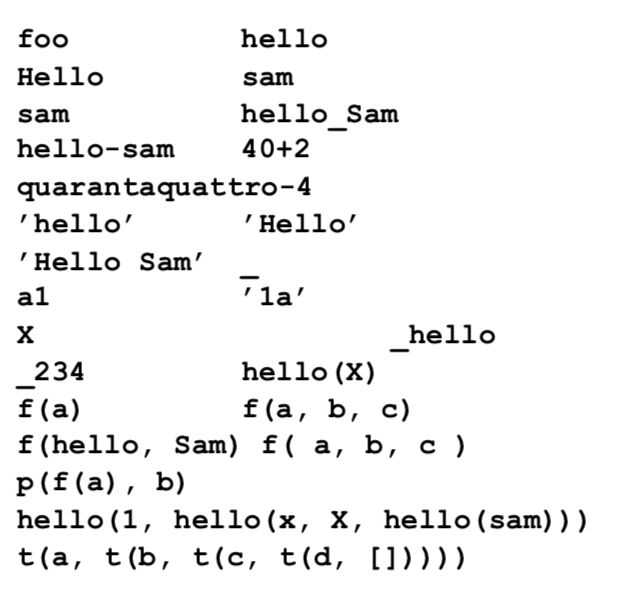
\includegraphics[width=0.75\textwidth]{validi}$$
Come si nota sono un po' di comandi a caso, ma privi di errori sintattici \\
{\color{black} \rule{\linewidth}{0.3mm} }
\\
Vediamo ora invece un esempio di comandi NON validi 
\\ \\
\textbf{Non validi} \\ \\
$$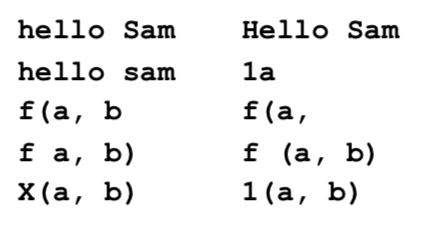
\includegraphics[width=0.75\textwidth]{nonvalidi}$$
In questo caso come vedete sono errori che tendenzialmente era possibile fare 
pure su Java, non è che si tratti di chissà che di complesso. \\
{\color{black} \rule{\linewidth}{0.3mm} }
\\
\\ \\
\subsection{Le variabili (logiche)}
La variabile logica è una sequenza alfanumerica che però inizia con un carattere
maiuscolo (oppure con l'Underscore \_), e se son composte solo dal simbolo \_ 
prendono il nome di Indifferenza o anonime.
\\ \\
Vengono instanziate (legate ad un valore) con il procedere del programma 
(Nella dimostrazione del teorema)
\subsection{Termini Composti}
In cosa consiste una composizione di termini? In un \color{red} funtore
\color{black} (Simbolo funzione, o predicato definito come atom) +
una sequenza di termini racchiusi tra parentesi tonde e separati da virgole.
Questi ultimi sono come gli argomenti dei metodi che facevamo in java, stesso
identico concetto. \\ \\
Non serve nemmeno essere uno spazio tra funtore e parentesi di sinistra, per 
via di caratteristiche del sistema di parsing di prolog
\section{Le Regole}
Sono utilizzabili per esprimere definizioni:
\begin{itemize}
	\item Se X è un animale ed X ha le squame, X è un pesce
\end{itemize}
Ms in modo informale una regola alla fine è una formula ben formata, ed è composta
da una testa e da un corpo (collegate da un operatore) quindi per ipotesi, una 
possibile regola potrebbe essere A :- B, concettualmente si legge A è 
implicata da B.
\\ \\
La testa di una regola è il conseguente di una implicazione logica, cioè quello 
che consegue dal corpo, che è appunto l'antecedente.
\begin{lstlisting}[language = Prolog]
A :- B
\end{lstlisting} 
si può tradurre in $B \to A$, ora proviamo a ritradurre il nostro
esempio del pesce:
\begin{lstlisting}[language = Prolog]
pesce(X) :- animale(x), ha_le_squame(X)
\end{lstlisting} 
In cui la virgola ovviamente è un and ($\wedge$) \\ \\
\paragraph{Attenzione: } già questo esempio presenta una vulnerabilità, nel senso
che per intenderci, essere un pesce implica di aver le squame, MA essere un 
animale ed avere le squame non implica essere un pesce.
\section{Regole di ricorsione}
Proviamo a definire il concetto di un antenato, che è l'esempio più semplice 
per capire come funzionano le formule ricorsive. Ci conviene ancora ragionare 
sulle nostre definizioni
\begin{lstlisting}[language = Prolog]
antenato(X, Y) :- genitore(X, Y).
antenato(X, Y) :- genitore(Z, Y), antenato(X, Z).
\end{lstlisting}
Traducendolo: \\
La prima riga si legge: \textbf{SE}~~~~ X è \color{red}genitore \color{black} di Y
\textbf{ALLORA} X è \color{red}antenato \color{black} di X. \\ \\
La seconda riga invece è appena appena più complessa, merita un ritorno a capo 
solo per lei: \\ \\
\textbf{SE}~~~~ X è \color{red}antenato \color{black} di Z \textbf{E} Z 
è \color{red}genitore \color{black} di Y \textbf{ALLORA} X è \color{red}antenato
 \color{black} di Y
\section{L'interprete prolog: Interrogazioni}
Come detto in precedenza possiamo chiamarle interrogazioni, query, goal, non sono
altro che comunicazioni dirette all'interprete che una volta fatto partire ci 
presenterà true o false. \\ \\
Un esempio di query:\\ 
\begin{lstlisting}[language = Prolog]
?- libro(kowalski, prolog).
\end{lstlisting}
Prolog ti restituirà come abbian detto prima true o false, yes o no, insomma ci
siamo capiti.
\\ \\
Volendo io posso interrogare anche il programma usando delle variabili esistenziali.
In pratica tutte le variabili Prolog le instanzia quando prova a darti una risposta,
e queste vengono mostrate nella tua risposta, per esempio:\\
libro(AUTORE, prolog) si legge come: CHI E' L'AUTORE DI PROLOG? 
(Un folle di sicuro, ma va be'.) \\ \\
\section{Unificazione: introduzione}
L'operazione di instanziazione di variabili durante la prova di un predicato è il 
risultato di una procedura particolare detta \textbf{Unificazione} \\ \\
Dati due termini, la procedura di unificazione crea un insieme di sostituzioni 
delle variabili, e questo insieme permette di rendere uguali i due termini. \\
\\ 
Tradizionalmente la procedura di unificazione costruisce un insieme di sostituzioni
che prende il nome di "Most general unifier (indicato con MgU" (No, fan della F1
non c'entra nulla con l'MGU-K o H :C)
\\ \\ 
Noi non faremo unificazioni, ci pensa l'interprete Prolog, che usa le 
unificazioni appunto. L'interprete Prolog stupido, che esegue algoritmicamente
operazioni semplici, deve tenere traccia di tutte le unificazioni, quindi rinomina
le variabili che userà durante il processo,
\\ \\
Come testiamo questa cosa? Prendiamo le due espressioni che vogliamo testare, le
poniamo con il simbolo uguale in mezzo, e ci darà il risultato. Possiamo chiedergli
42 = 42? e 42=x e ci dà yes in entrambi questi casi
\subsection{Most General Unifier} 
E' il risultato finale della procedura di valutazione, o meglio, di prova del 
Prolog. \\
Il modo più comodo per vedere appunto come la procedura di unificazione funziona 
è di usare l'=
\section{Le Liste in Prolog: }
Si definisce una lista in Prolog racchiudendo gli elementi (termini e/o variabili logiche) della lista tra parentesi quadre

‘[’ e ‘]’ e separandoli da virgole.
Gli elementi di una lista in Prolog possono essere termini qualsiasi o liste
[] indica la lista vuota.
\\ \\
Ogni lista non vuota può essere divisa in due parti, la testa e la coda, che sono
rispettivamente il primo elemento e "tutti gli altri". Un po' come in F1, la 
testa è la Mercedes, la coda son tutte le altre squadre (O la Juve in Serie A
negli ultimi anni).
\end{document}